%	현대물리실험 보고서
%	실험2
%	202100973 이승엽

%----------------------------------------------------------------------------------------
%	PACKAGES AND DOCUMENT CONFIGURATIONS
%----------------------------------------------------------------------------------------

\documentclass[a4paper, 10pt, nanum]{CSUniSchoolLabReport}
% use UTF8 encoding
\usepackage[utf8]{inputenc}
% use KoTeX package for Korean
\usepackage{kotex}
\usepackage{amsmath}
\usepackage{hyperref}
\usepackage{graphicx}
\usepackage{indentfirst}
\usepackage{setspace}
\usepackage{multirow}
\usepackage{enumitem}
\usepackage{graphicx}
\usepackage{wrapfig}
\usepackage{epstopdf}
\usepackage{caption}
\usepackage{subcaption}

\setlength{\parindent}{0.2in} % 들여쓰기 길이 설정
\setlength{\parskip}{3mm} % 문단 간의 간격 조절
\setstretch{1.5} % 줄간격

\addbibresource{reference.bib} % Bibliography file (located in the same folder as the template)

%----------------------------------------------------------------------------------------
%	REPORT INFORMATION
%----------------------------------------------------------------------------------------

\title{현대물리실험 실험2 보고서 \\ 3D Printing} % Report title

\author{\textsc{Department of Physics} 202100973 이승엽}

\date{\today}

%----------------------------------------------------------------------------------------

\begin{document}

\maketitle % Insert the title, author and date using the information specified above

\begin{center}
	\begin{tabular}{l r}
		Date Performed: & April 11, 2023 \\ % Date the experiment was performed
		& April 18, 2023 \\
		Partners: & 202100969 이규리 \\ % Partner names
		& 202100989 한누리 \\
		Instructor: & Professor 이기주 \\ % Instructor/supervisor
		Typesetting: & LaTeX \\
	\end{tabular}
\end{center}

%----------------------------------------------------------------------------------------
%	ABSTRACT
%----------------------------------------------------------------------------------------

\maketitle
% \begin{abstract}
% 	This report ...
% \end{abstract}

%----------------------------------------------------------------------------------------
%	INTRODUCTION
%----------------------------------------------------------------------------------------

\section{서론}

	무엇무엇

%----------------------------------------------------------------------------------------
%	THEORY
%----------------------------------------------------------------------------------------

\section{이론}

	3D 프린터는 여러 종류가 있으나, 실험에서 사용하는 프린터는 Sindoh X1이다. 이 프린터는 필라멘트를 바닥면부터 위로 층층이 쌓는다. 
	\begin{figure}[htb!]
		\centering
		\includegraphics[width=5cm]{fig1.png}
		\caption{3D Printer, Sindoh X1}
		\label{fig:1}
	\end{figure}

%----------------------------------------------------------------------------------------
%	EXPERIMENTAL METHOD
%----------------------------------------------------------------------------------------

\section{실험 방법}

\subsection{컵}

\begin{enumerate}[label=\arabic*.]
	\item 123D DESIGN tool을 사용하여 3-D modeling을 디자인한다. (교재를 참고한다.)
	\begin{figure}[htb!]
		\centering
		\begin{minipage}{.5\textwidth}
			\centering
			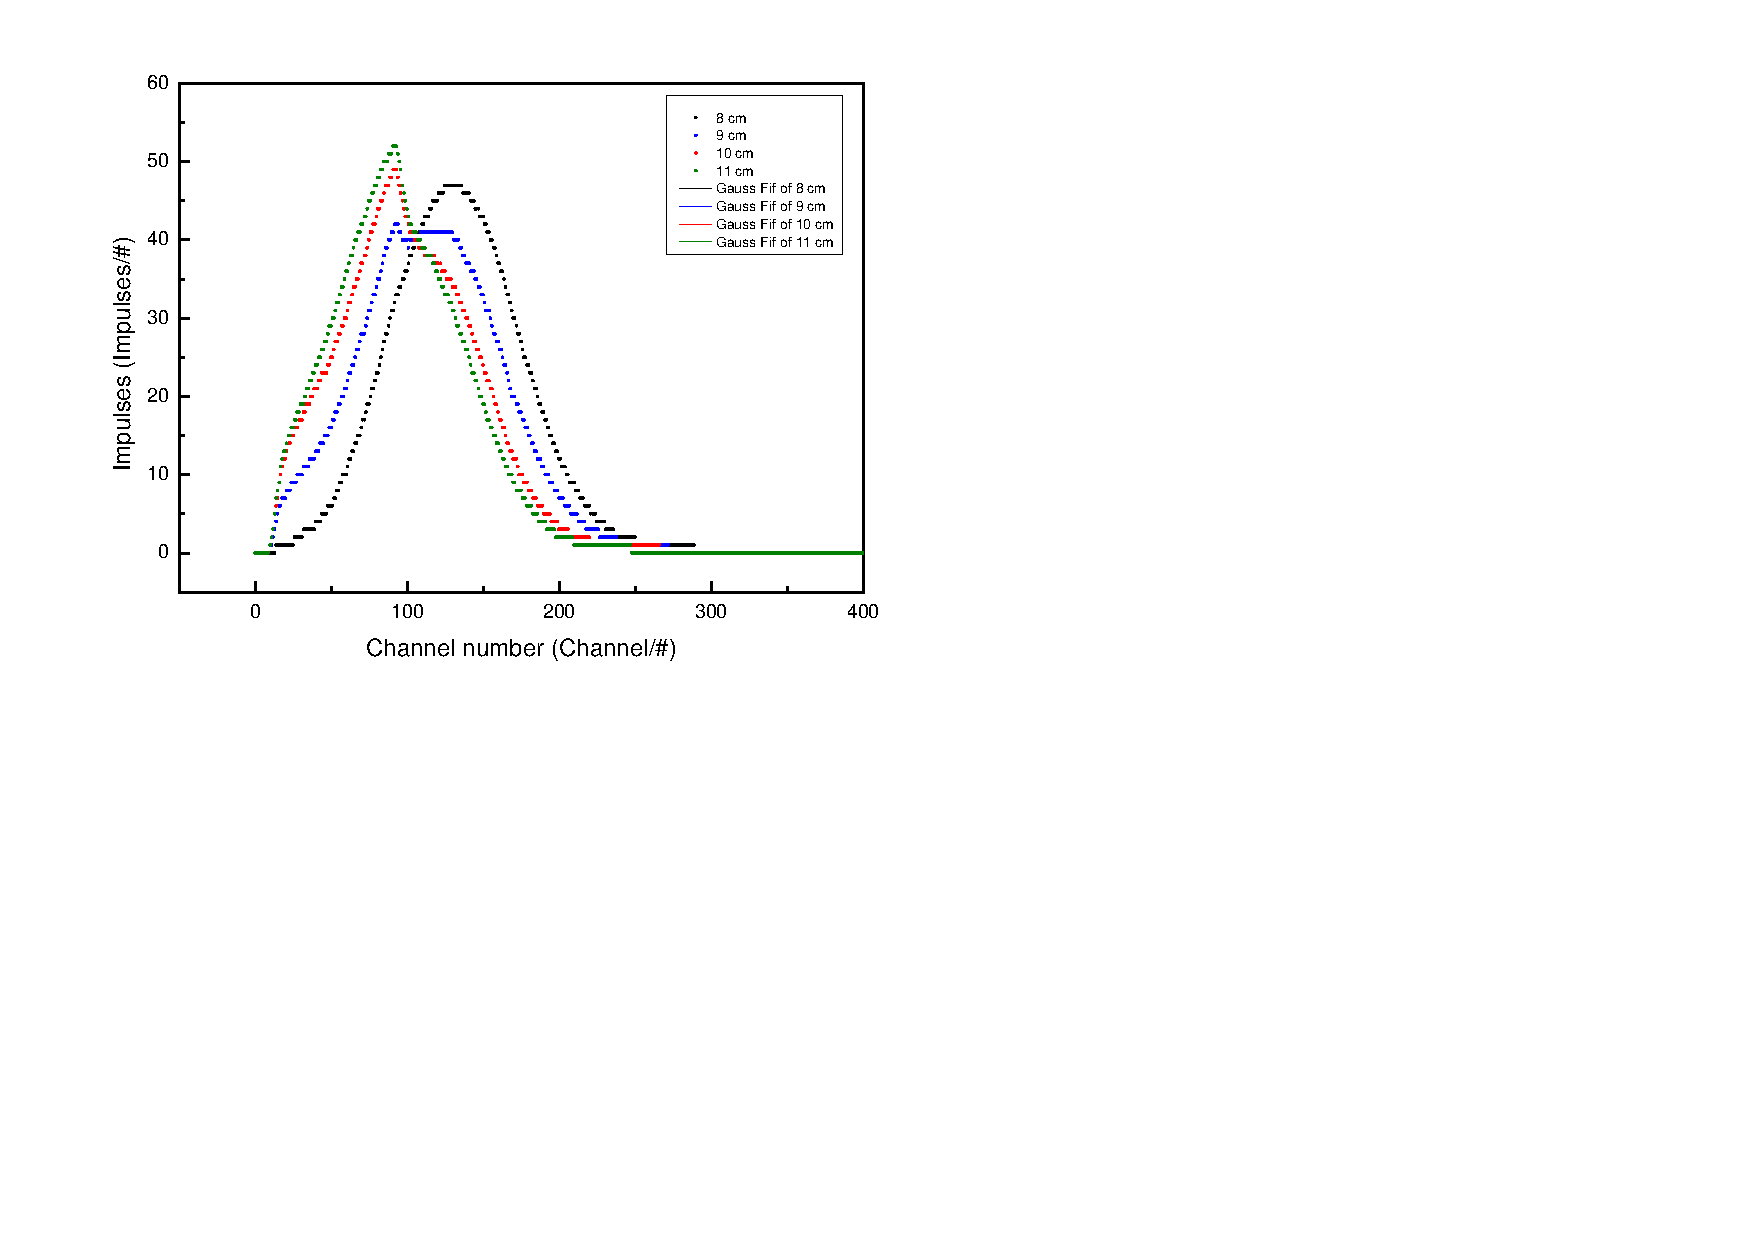
\includegraphics[width=5cm]{fig2.jpg}
			\captionof{figure}{3D modeling}
			\label{fig:2}
		\end{minipage}%
		\begin{minipage}{.5\textwidth}
			\centering
			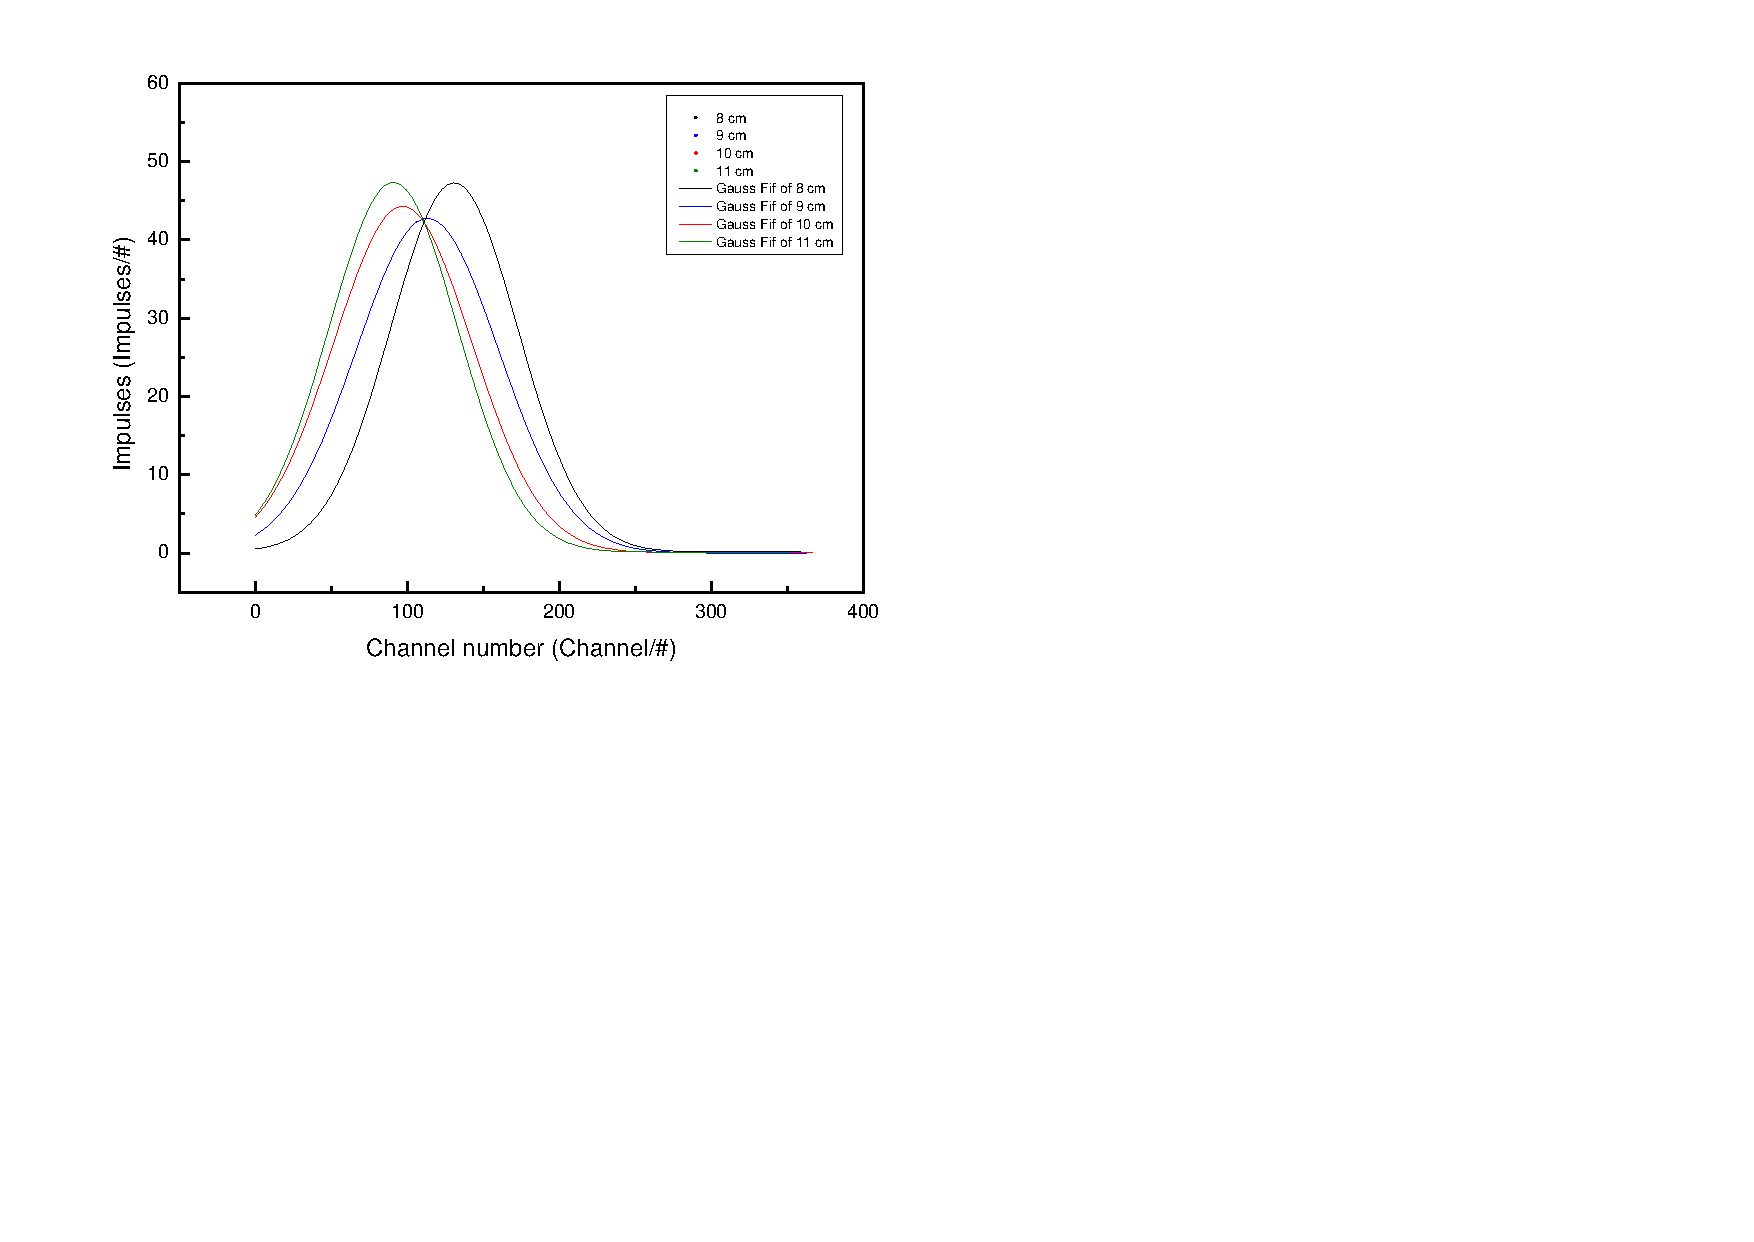
\includegraphics[width=5cm]{fig3.jpg}
			\captionof{figure}{3D modeling}
			\label{fig:3}
		\end{minipage}
	\end{figure}
	\begin{figure}[htb!]
		\centering
		\begin{minipage}{.5\textwidth}
			\centering
			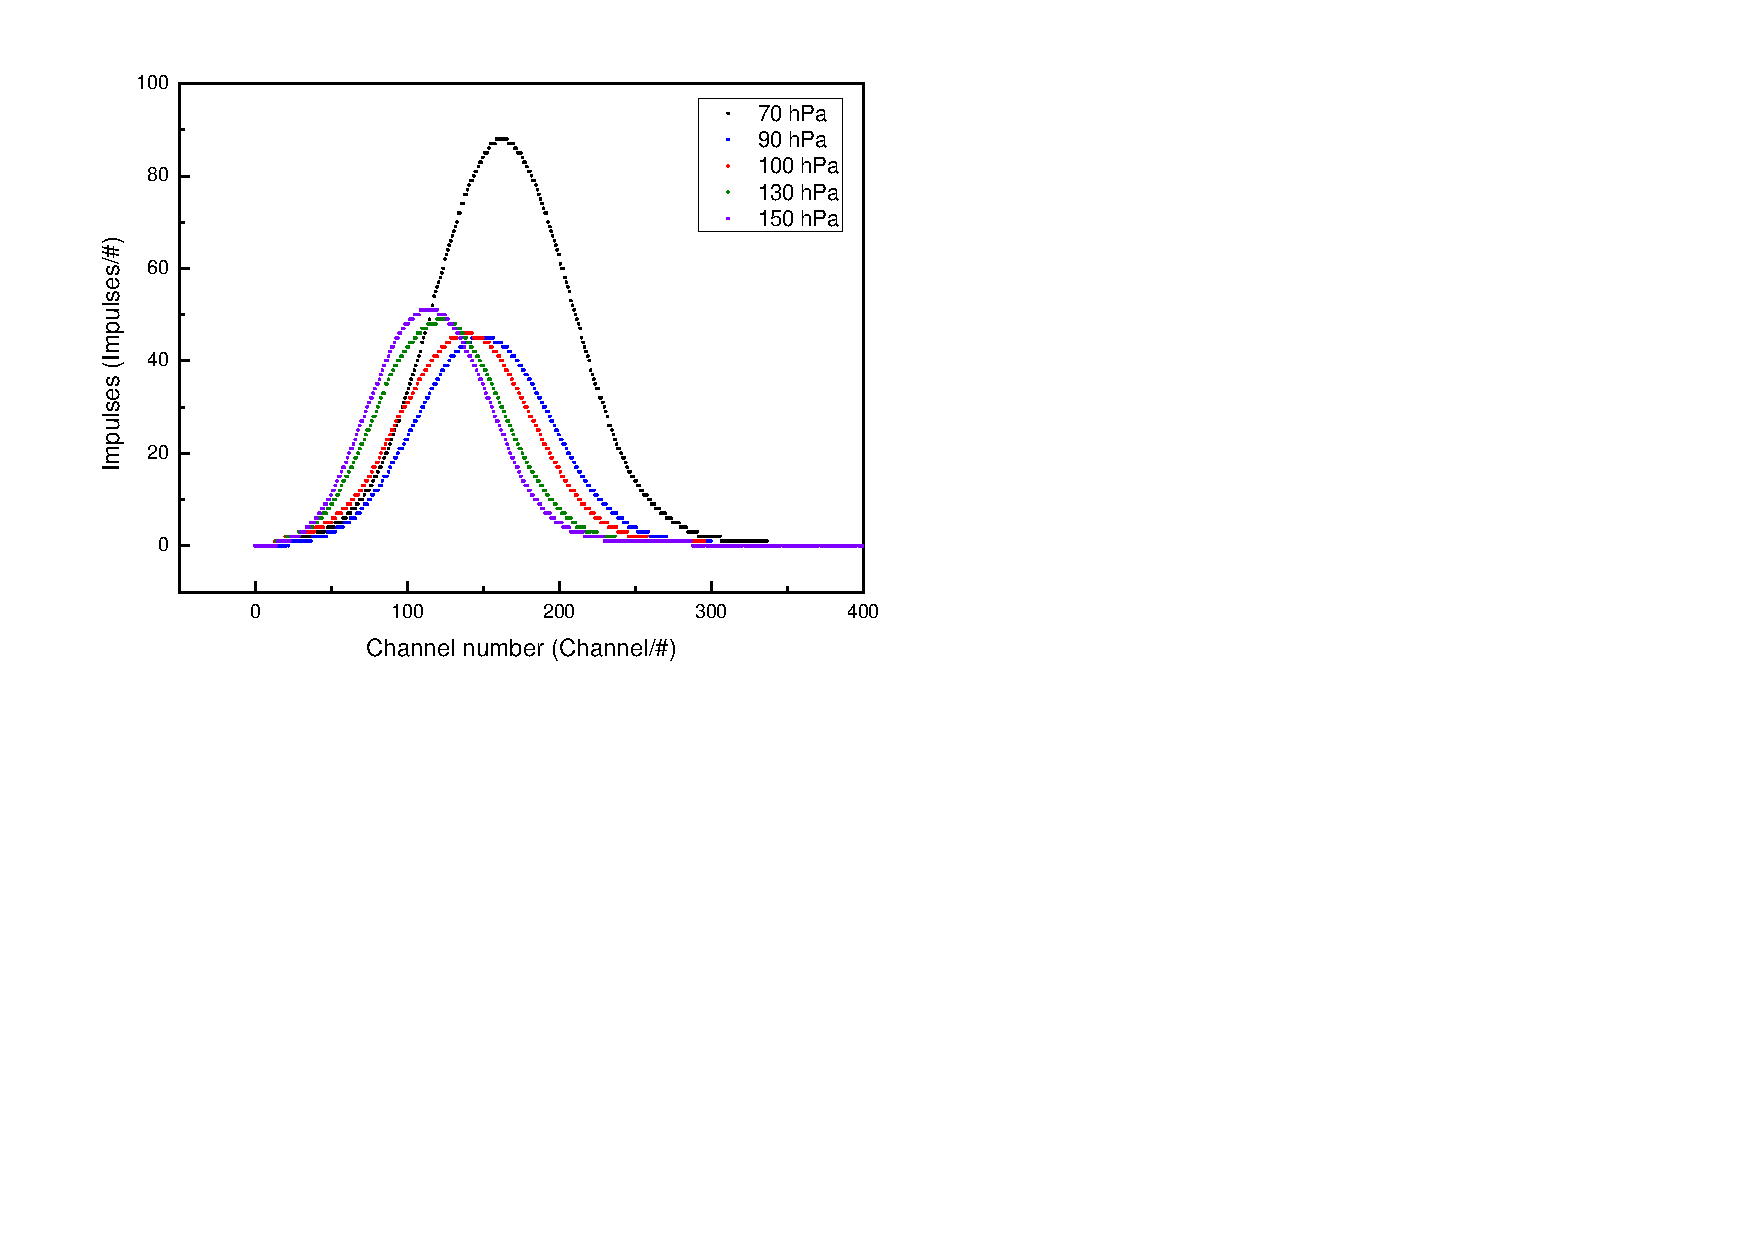
\includegraphics[width=5cm]{fig4.jpg}
			\captionof{figure}{3D printing}
			\label{fig:4}
		\end{minipage}%
		\begin{minipage}{.5\textwidth}
			\centering
			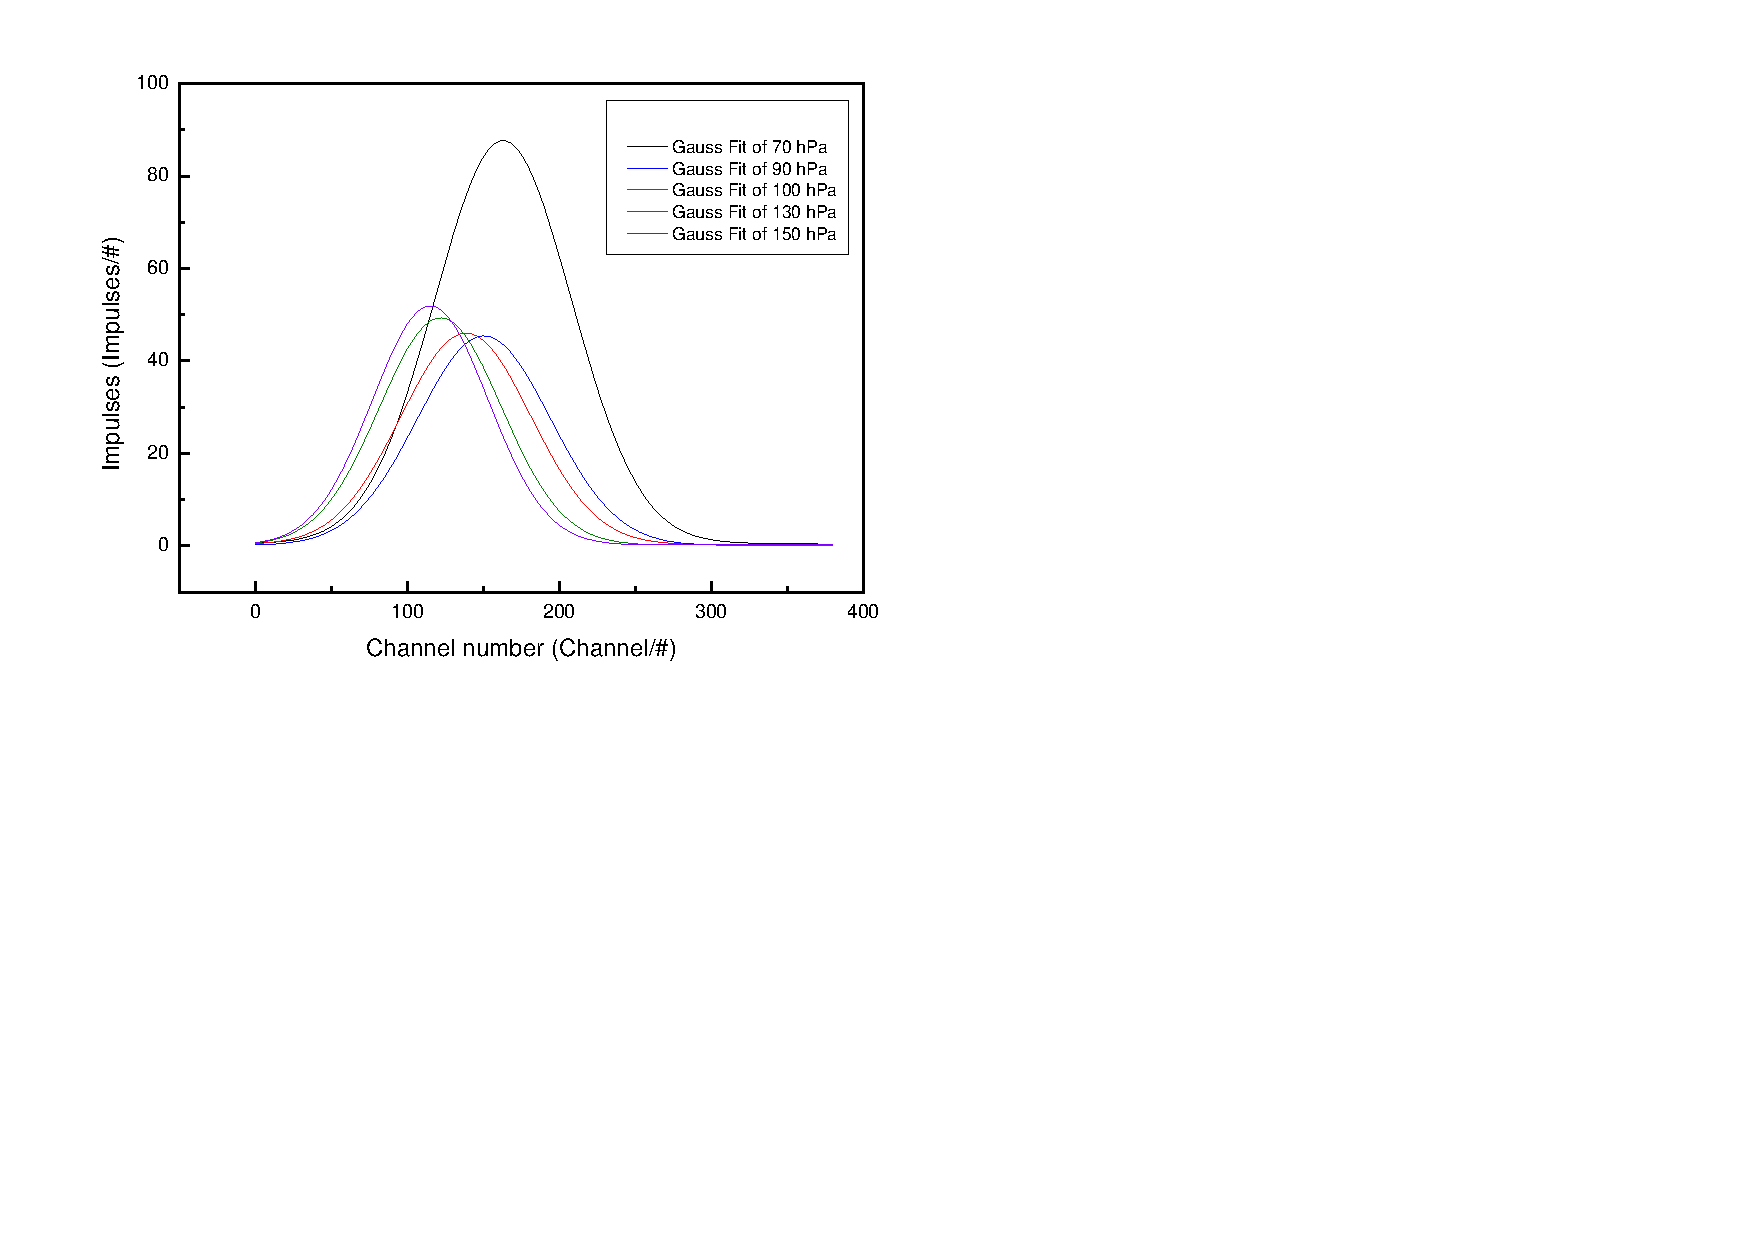
\includegraphics[width=5cm]{fig5.jpg}
			\captionof{figure}{3D printing}
			\label{fig:5}
		\end{minipage}
	\end{figure}
	\begin{figure}[htb!]
		\centering
		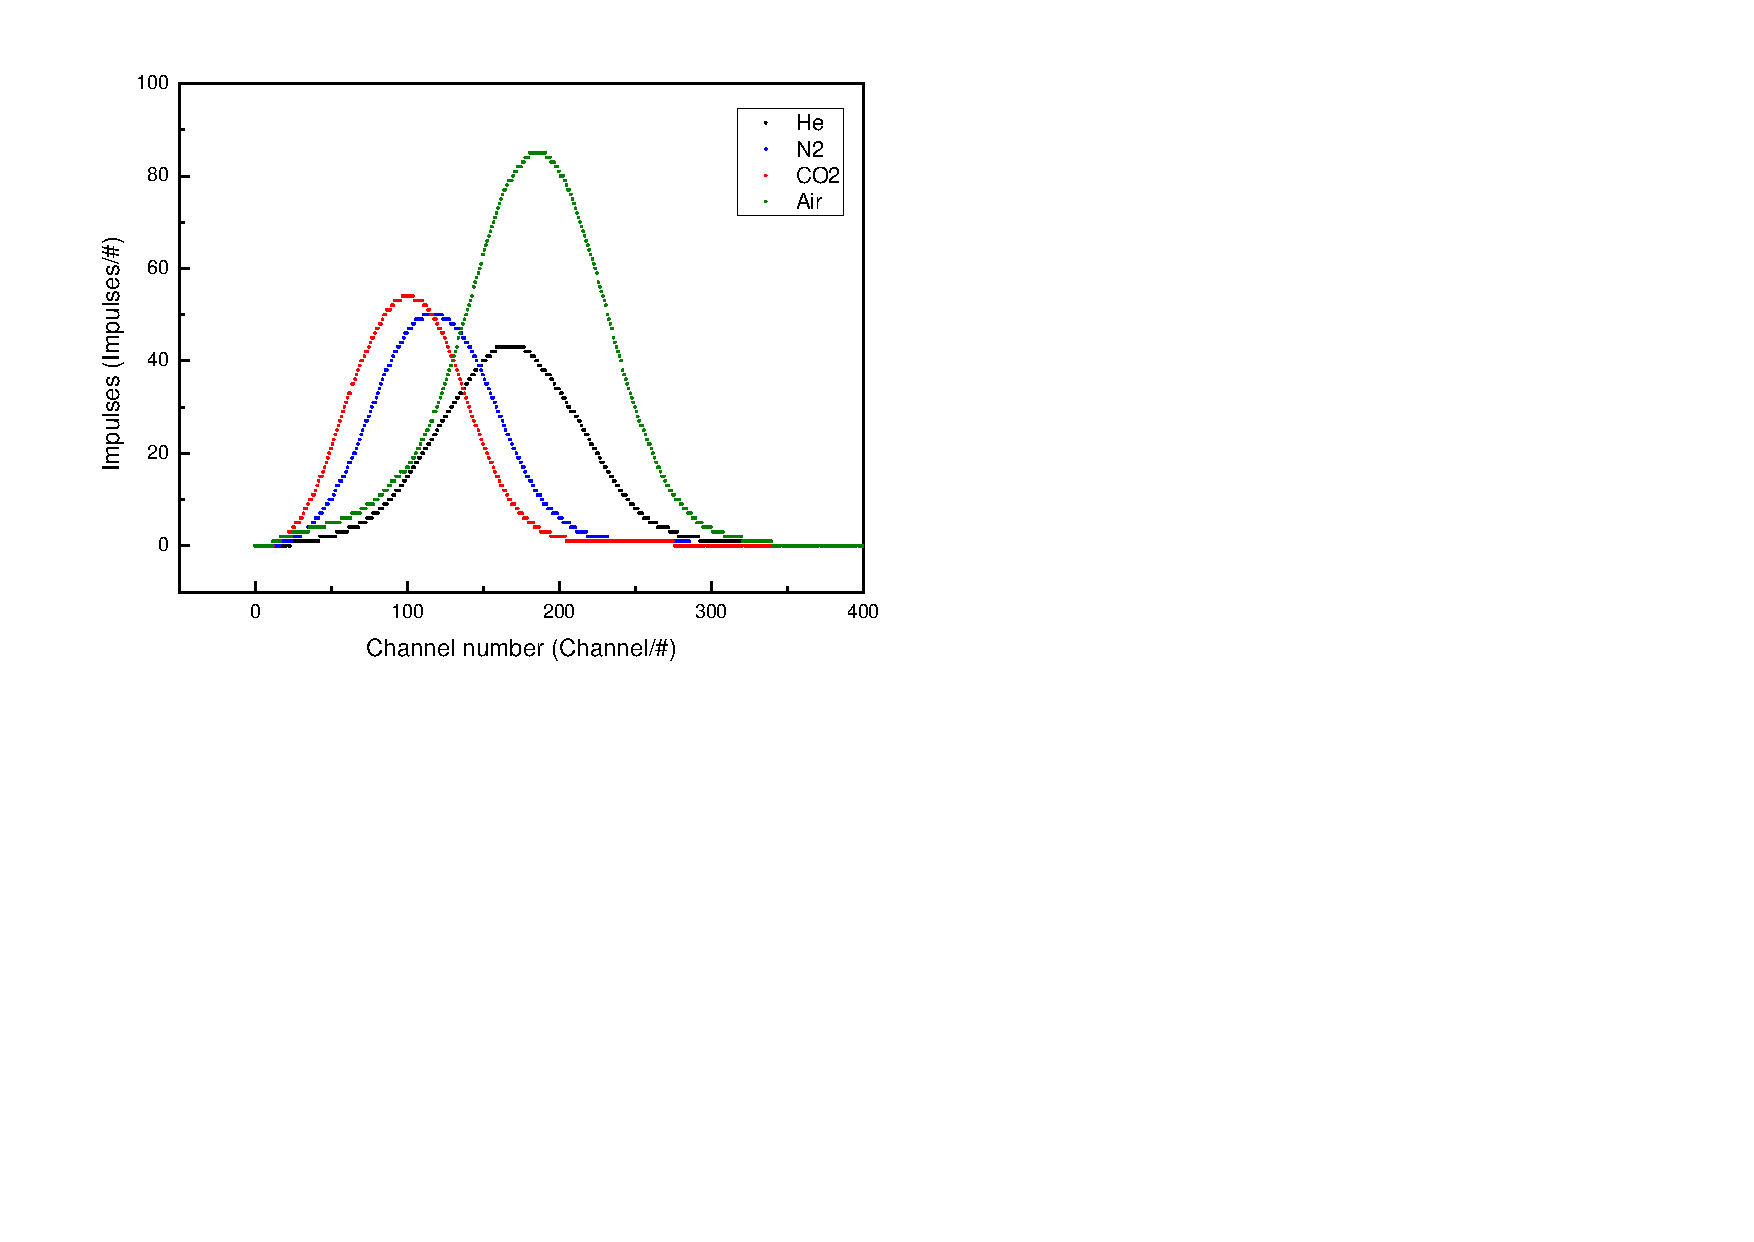
\includegraphics[width=5cm]{fig6.jpg}
		\caption{3D model}
		\label{fig:6}
	\end{figure}
\end{enumerate}

\subsection{왕관}

\begin{enumerate}[label=\arabic*.]
	\item 123D DESIGN tool을 사용하여 3-D modeling을 디자인한다.
	\item 반지름이 20 mm인 원기둥(C$_1$)을 만든 후, 원기둥의 가장 높은 옆면 부분에 반지름이 10 mm이고 90도로 기운 원기둥(C$_2$)을 360도 전 면에 붙인다.
	\item C$_2$을 C$_1$의 안쪽으로 일부를 넣어 왕관의 날카로운 부분을 구상한다.
	\item C$_1$을 C$_2$ 묶음으로 차집합하여 왕관의 날카로운 모양을 만든다.
	\item C$_1$의 내부를 비우기 위해 C$_1$보다 2 mm 작은 원기둥을 만든 후 차집합한다.
	\begin{figure}[htb!]
		\centering
		\begin{minipage}{.5\textwidth}
			\centering
			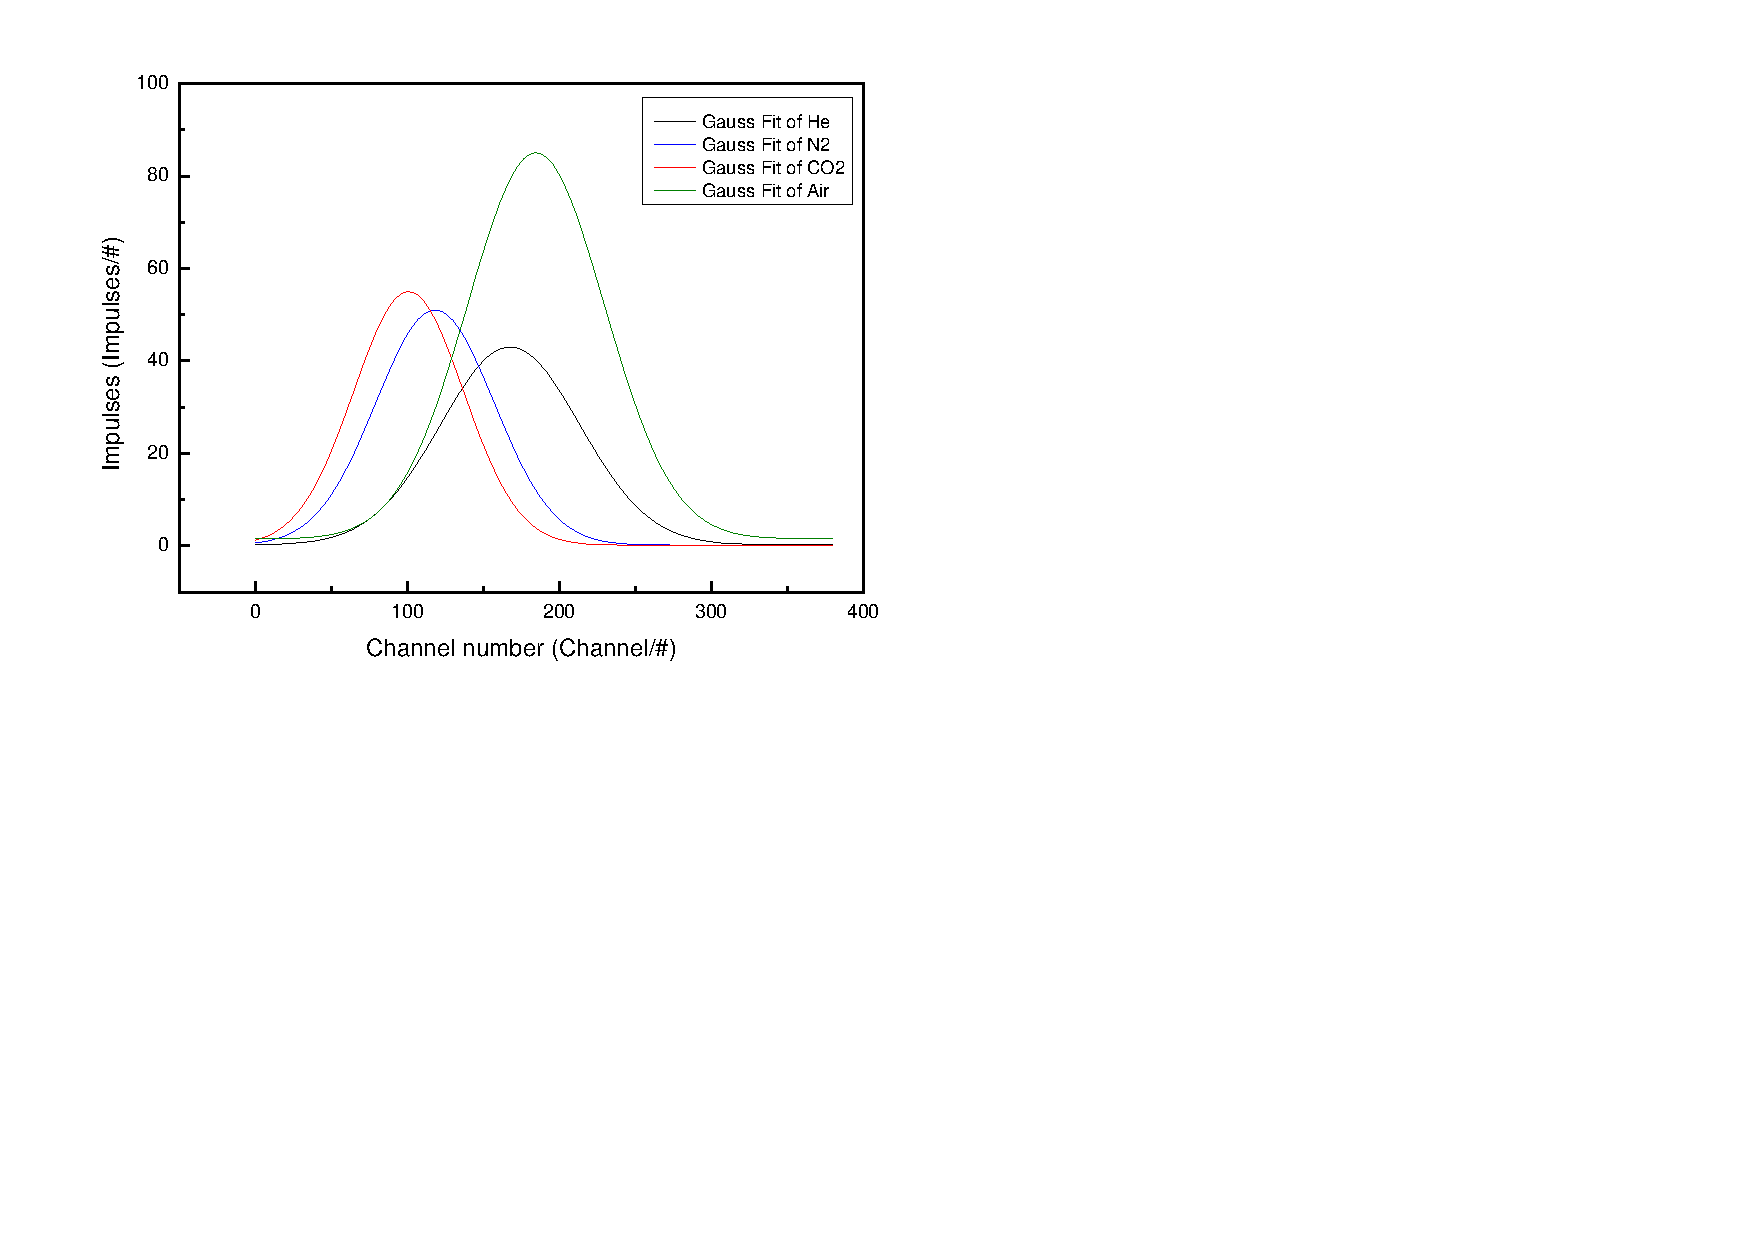
\includegraphics[width=5cm]{fig7.jpg}
			\captionof{figure}{3D modeling}
			\label{fig:7}
		\end{minipage}%
		\begin{minipage}{.5\textwidth}
			\centering
			\includegraphics[width=5cm]{fig8.jpg}
			\captionof{figure}{3D printing}
			\label{fig:8}
		\end{minipage}
	\end{figure}
\end{enumerate}

%----------------------------------------------------------------------------------------
%	RESULT AND DISCUSSION
%----------------------------------------------------------------------------------------

\section{실험 결과}

	작은 크기로 왕관을 모델링하여 프린팅하였다. 크기가 작고 기기의 한계로 인하여 마감 상태가 고르지 않고, 높이가 모델링한 것과 실제 사이즈와 오차를 보였다.

	\begin{figure}[htb!]
		\centering
		\includegraphics[width=5cm]{fig9.jpg}
		\caption{3D model}
		\label{fig:9}
	\end{figure}


%----------------------------------------------------------------------------------------
%	CONCLUSIONS
%----------------------------------------------------------------------------------------

\section{결론}

	3D 모델링과 프린팅을 해 보았고, 크기가 큰 것을 제작함에 있어 시간에 비례하나 작게할 경우 마감이 깔끔하지 못함을 알 수 있다. 더 정밀한 마감을 원할 경우 더 좋은 기기를 사용하거나 모델 사이즈를 키워 상대적 오차를 줄이는 방법을 사용하면 될 것이다.

%----------------------------------------------------------------------------------------
%	BIBLIOGRAPHY
%----------------------------------------------------------------------------------------

% \printbibliography % Output the bibliography

%----------------------------------------------------------------------------------------

\end{document}